\documentclass[a4paper, 10pt]{article}
\usepackage[utf8]{inputenc}
%\usepackage[brazil]{babel}
\usepackage[top=3cm,left=3cm,right=2cm,bottom=2cm]{geometry} % para as margens
\usepackage{graphicx} % para as figuras  
\usepackage{color}
\usepackage[hidelinks]{hyperref}
\usepackage{listings}

% ---------------------------------------------------------------------------- %
% Macros for proof-reading
\usepackage{color}
\usepackage{xcolor}
\usepackage[normalem]{ulem} % for \sout
\newcommand{\ugh}[1]{\textcolor{red}{\uwave{#1}}} % please rephrase
\newcommand{\ins}[1]{\textcolor{blue}{\uline{#1}}} % please insert
\newcommand{\del}[1]{\textcolor{red}{\sout{#1}}} % please delete
\newcommand{\chg}[2]{\textcolor{red}{\sout{#1}}{$\rightarrow$}\textcolor{blue}{\uline{#2}}} % please change

% Put edit comments in a really ugly standout display
\usepackage{ifthen}
\usepackage{amssymb}
\newboolean{showcomments}
\setboolean{showcomments}{true} % toggle to show or hide comments
\ifthenelse{\boolean{showcomments}}
  {\newcommand{\nb}[2]{
    \fcolorbox{gray}{yellow}{\bfseries\sffamily\scriptsize#1}
    {\sf\small$\blacktriangleright$\textit{#2}$\blacktriangleleft$}
   }
   \newcommand{\version}{\emph{\scriptsize$-$working$-$}}
  }
  {\newcommand{\nb}[2]{}
   \newcommand{\version}{}
  }

% General comment
\newcommand\info[1]{\nb{Info}{#1}}
\newcommand\todo[1]{\nb{ToDo}{#1}}

% Single author comment
\newcommand\Gerosa[1]{\nb{Gerosa}{#1}}
\newcommand\Fabio[1]{\nb{Fabio}{#1}}
\newcommand\Leo[1]{\nb{Leo}{#1}}
\newcommand\gerosa[1]{\nb{Gerosa}{#1}}
\newcommand\fabio[1]{\nb{Fabio}{#1}}
\newcommand\leo[1]{\nb{Leo}{#1}}


\newcommand{\ee}{Enactment Engine}
\newcommand{\cd}{Choreography Deployer}
\newcommand{\dm}{Deployment Manager}

\title{CHOReOS \ee\ Installation Guide}
\author{Leonardo Leite (IME - USP)}

\begin{document}

\maketitle

\section{Introduction}

The CHOReOS \ee\ provides a Platform as a Service (PaaS) that automates the distributed deployment of service choreographies in cloud environments. This document provides instructions about how to install, configure, and run the \ee.

We will describe now each one of the \ee\ components, that are pictured in the Fig.~\ref{fig:ee_components}. The \cd\ and the \dm\ are components provided by the \ee, whereas the Chef components and the Cloud Gateway are third-party software used by the \ee.

\begin{figure}
\centering
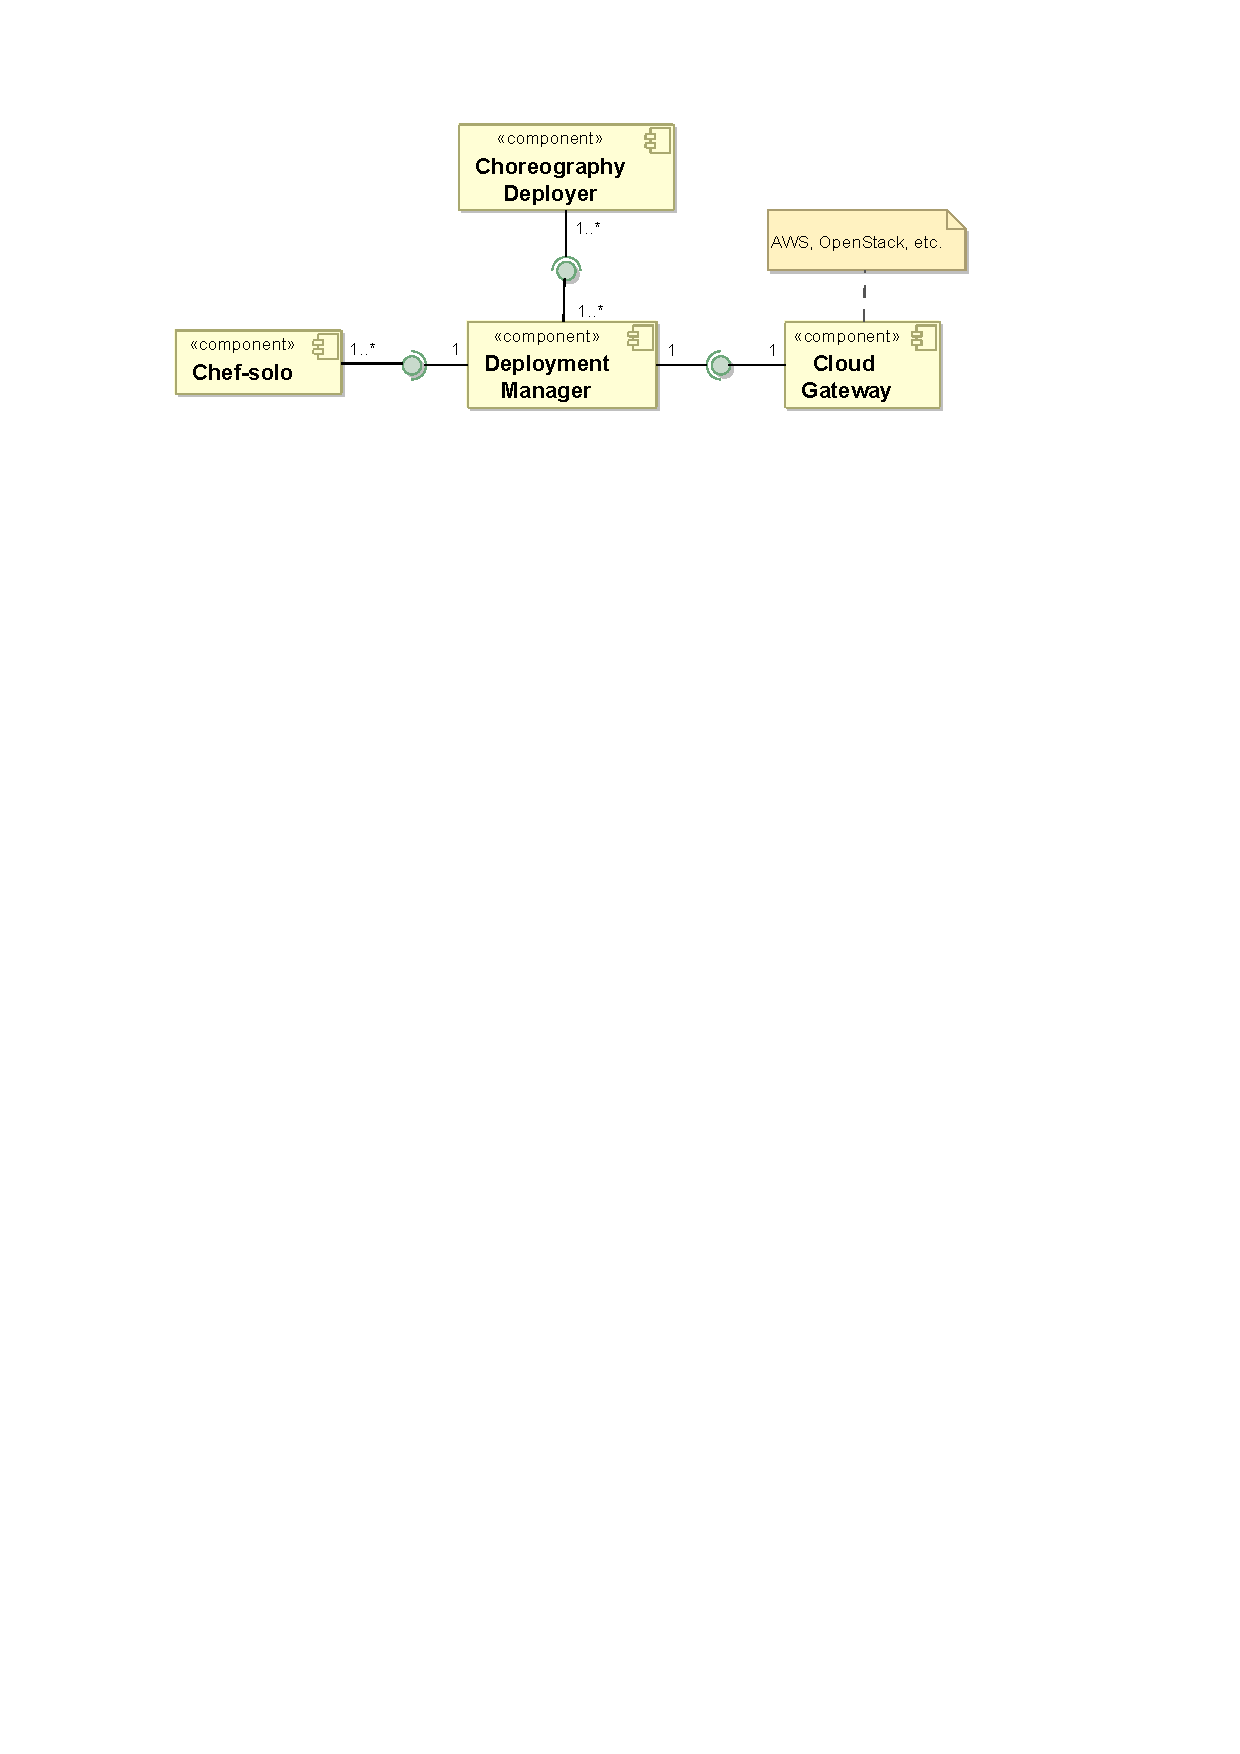
\includegraphics[scale=0.7]{img/components.pdf}
\caption{\ee\ architecture}
\label{fig:ee_components}
\end{figure}

\begin{description}

\item [Cloud Gateway] creates and destroys virtual machines (also called \emph{nodes}) in a cloud computing environment. This component is used by the \dm, that decides when create or destroy the nodes. Currently, only Amazon EC2 and OpenStack are supported as Cloud Gateways, but the \dm\ may be extended to support other virtualization technologies.

\item [Chef Server:] in an environment managed by Chef, nodes software configuration are specified by ``recipes'', that are scripts written in a Ruby-like Domain Specific Language. In the \ee, recipes implement the process of configuring operational system, installing required middleware, and finally deploying the services. The recipes and the association between recipes and nodes are stored on Chef Server.

\item[Chef Client] is installed by the \ee\ in each managed node. It uses the Chef Server REST API to retrieve the recipes that are associated to the local node and update the node software configuration by executing the recipes. 

\item [\dm] deploys services in a cloud environment. Through its REST API, the \dm\ receives a declarative service specification and selects the node where the service will be deployed, possibly considering the service non-functional requirements. The \dm\ converts the received specification into a Chef recipe that implements the service installation process. After generating the recipe, the \dm\ stores on the Chef Server the generated recipe and the association between the recipe and the selected node. Using other \dm\ REST operation, one can request the upgrade of a node, which consists in running the Chef Client on that node.

\item [\cd] exposes the REST API to web service choreography automated deployment. The \cd\ client must provide a choreography declarative specification, that contains the choreography architectural description and the locations of service packages. Based on this specification, the \cd\ coordinates invocations to the multiple \dm{s} belonging to the different participant organizations. After services deployment, the \cd\ provides the provider services locations to their respective consumer services.

\end{description} 


In this guide we assume that both \cd\ and \dm\ components will be executed on the deployer machine. Deployer is the human operator responsible by the deployment process. For while, a \cd\ instance is limited to use only one \dm.

\section{Requirements}

Before you run \ee, you will need:

\begin{itemize}
\item SVN;
\item Java 6 (we are using OpenJDK);
\item Maven 3  (\url{http://maven.apache.org/download.html});
\item a Cloud Gateway access, as detailed in Section~\ref{sec:cloud};
\item a Chef account, as detailed in Section~\ref{sec:chef}.
\end{itemize}

\section{Cloud Provider}
\label{sec:cloud}

A \textsf{CloudProvider} is an \ee\ interface that specifies methods to CRUD virtual machines. It is expected that a \textsf{Cloud Provider} implementations will act just as a client of some Cloud Gateway. In this section we describe the currently available \textsf{CloudProvider} implementations and how to use them. New \textsf{CloudProvider}s may be implemented to support other virtualization tools. One example would be creating a \textsf{VirtualBoxCloudProvider} to create VMs using VirtualBox.

Whatever the cloud provider you choose, ensure that the required TCP ports of the created VMs are unblocked. Required ports: 22 to SSH, 8080 to Tomcat, the Chef Server port (for us it is 4000), the ports used by your JAR services, and the port 8180 to EasyESB.

\subsection{Amazon EC2}

Amazon EC2 service is the simplest choice to dynamically retrieve VMs as you need. You need just to create an account at \url{http://aws.amazon.com} and configure a pair of keys to access the VMs through SSH. The trade-off is that you must to pay to Amazon! 

Some hints:

\begin{itemize}
\item Request credits to education purposes: \url{http://aws.amazon.com/grants/}. The first of us earned \$500, but the others \$100. Maybe it depends on your research project description.
\item Initially there is a limit of 20 VMs that you can run simultaneously.
\item Request to increase Amazon EC2 instance limit: \url{http://aws.amazon.com/contact-us/ec2-request/}. At USP we got a 50 VMs limit.
\item Pay attention to the ``one-second rule'': \\ \url{http://www.a2sdeveloper.com/page-working-with-the-one-second-rule.html}.
\item As we are charged per hour, don't forget to shutdown/stop unused VMs.
\item You can use the Amazon EC2 web console to unblock TCP ports necessary to the choreography execution.
\item You can also use the \texttt{ec2} command line tools to manage your VMs.
\item The \ee\ creates VMs in the ``US East'' Amazon datacenter.
\item The SSH keypairs are datacenter-dependent. Therefore if you create a keypair in the EU
datacenter, it won't be valid for your VMs.
\end{itemize}

\subsection{OpenStack}

OpenStack is an open source private cloud platform that provides services to retrieve VMs as you need, in the same way that Amazon EC2. However, you must install OpenStack in your own infrastructure, which means you must own at least a little cluster (or a very powerful machine) to host the created VMs. Moreover, the OpenStack installation and configuration is not a simple task.

Some hints:

\begin{itemize}
\item OpenStack does not provide public IPs, therefore some VPN configuration is necessary to log into the provisioned nodes.
\item you can also use the \texttt{nova} command line tool to manage your VMs.
\end{itemize}

\subsection{Fixed cloud provider}

If you are learning how to use the \ee\ and want just to experiment it, the \textsf{FixedCloudProvider} may be best possible to you. With it you are responsible to manually crating and setting virtual machines and telling to \ee\ which machines must be used by it. This avoids the overhead of dealing with a cloud environment. 

When creating a virtual machine to be used by the \ee, be sure:
\begin{itemize}
\item to use the Ubuntu 12.04 as operating system;
\item it is possible to SSH into the node without typing a password: \url{http://www.integrade.org.br/ssh-without-password}\footnote{Obs: do not use a key with password.};
\item use sudo in the machine without typing a password: type \texttt{\$sudo visudo} and add the line \texttt{<user> ALL = NOPASSWD: ALL} at the end (change \texttt{<user>} by the actual user);
\item to synchronize the machine clock: \texttt{\#ntpdate ccsl.ime.usp.br};
\end{itemize}

Configure the \texttt{deployment.properties} file settings according to the template.

To verify if your VM was properly set, you may run the \\ \textsf{org.ow2.choreos.deployment.nodes.cloudprovider.FixedConnectionTest} test.

When you use the \ee\ to install a service in your VM, the \ee\ will take care of bootstrapping (installing Chef) on your VM. The bootstrap process may take a few minutes. Therefore, saving a VM snapshot just after the bootstrap may save you a lot of time, since you can quickly restore your VM to a clear state. You may also bootstrap your VM by running the \textsf{ow2.choreos.deployment.nodes.NodeBootstrapperTest} test.

After testing and installing some recipes in the VM, you can restore the bootstrapped snapshot (as well as any other you have) by manually doing it in your preferred virtualization software (e.g. VirtualBox) and resetting the chef node run list. The last step can be easily done using the script \texttt{chef-repo/run\_list\_reset.sh}. You must create the \texttt{chef-repo/run\_list\_reset.conf} script according to the template (\texttt{run\_list\_reset.conf.template}).

Depending on how you create your VMs, some network configuration may be needed. In case of using VirtualBox, you can refer to \url{http://ccsl.ime.usp.br/foswiki/bin/view/Choreos/VMs}.

\section{Chef}
\label{sec:chef}

\dm\ will properly configure the nodes using Chef, an open-source configuration management system. With Chef you can specify a resources set to be deployed into cloud nodes. These resources are described by a Ruby-like DSL (Domain Specific Language), and include: systems, files, scripts execution, and others.

You can setup your own Chef server, or create an Hosted Chef server account. Hosted Chef is offered by Opscode\footnote{\url{http://www.opscode.com/}}. Although Hosted Chef frees you from setting the Chef Server in the infrastructure of your organization, it allows only a limited number of nodes to be managed by Chef.

Make sure your \texttt{knife.rb} file be something like the example on Listing~\ref{lst:kniferb}. You can use the template in \texttt{chef-repo/.chef/knife\_template.rb} to create your \texttt{knife.rb}, that should stay in the \texttt{.chef} directory.

{\footnotesize
\begin{lstlisting}[caption=knife.rb example,label=lst:kniferb] 
log_level                :info 
log_location             STDOUT 
node_name                "lleite" 
client_key               "#{current_dir}/lleite.pem" 
validation_client_name   "choreos-verao-validator" 
validation_key           "#{current_dir}/choreos-verao-validator.pem" 
chef_server_url          "https://api.opscode.com/organizations/choreos-verao" 
cache_type               'BasicFile' 
cache_options( :path => "#{ENV['HOME']}/.chef/checksums" ) 
cookbook_path            ["#{current_dir}/../cookbooks"] 
\end{lstlisting}
}

Here, the ``node\_name'' corresponds to my \emph{client} name. Make sure your client is marked as ``admin'', what can be accomplished by using the Chef Server web interface.  The  ``choreos-verao" is the organization name configured on the Chef Server. In the Chef terminology, your computer, from where you control Chef, is the \emph{workstation}. To more details about how to set up your workstation, refer to \url{http://wiki.opscode.com}. You will also need to upload to your Chef Server all the cookbooks from our cookbook folder: \texttt{chef-repo/cookbooks}.


\section{Checkout and Compilation}

To checkout the code: \texttt{svn checkout svn://svn.forge.objectweb.org/svnroot/choreos/trunk/cloud cloud}. 

After installing Maven 3, open the terminal at the \texttt{choreos\_middleware} folder, and run the \texttt{build.sh} script. It can take several minutes. Internet access is necessary during compilation.

\section{Configuration}

Open the folder \texttt{DeploymentManager/src/main/resources}, and create a \texttt{deployment.properties} file by copying the \texttt{deployment.properties.template} file. The new properties file must be created in the same folder. Open the just created properties file and edit it following instructions on the template file. The Listing~\ref{lst:deployment_properties} shows an example. Do the same process to the template properties file in \texttt{ChoreographyDeployer/src/main/resources}.

\lstset{
numbers=left
}

{\footnotesize
\begin{lstlisting}[caption=deployment.properties example,label=lst:deployment_properties] 
NODE_POOL_MANAGER_PORT=9100
SERVICE_DEPLOYER_PORT=9101
NODE_SELECTOR=ROUND_ROBIN
CLOUD_PROVIDER=AWS
FIXED_VM_IP=192.168.56.102
FIXED_VM_HOSTNAME=choreos-node
FIXED_VM_PRIVATE_SSH_KEY=/home/leonardo/.ssh/nopass
FIXED_VM_USER=choreos
AMAZON_ACCESS_KEY_ID=AKIAIIT2fsdfISddSECRETEFJH6Q
AMAZON_SECRET_KEY=N+KzHQITaALSOwzfdsAj9MiSECRETE0UPuwyD
AMAZON_KEY_PAIR=leofl
AMAZON_PRIVATE_SSH_KEY=/home/leonardo/.ssh/leofl.pem
CHEF_CONFIG_FILE=/home/leonardo/chef/chef-repo/.chef/knife.rb
CHEF_REPO=/home/leonardo/chef/chef-repo
\end{lstlisting}
}

Options to CLOUD\_PROVIDER: AWS, OPEN\_STACK, and FIXED.

Options to NODE\_SELECTOR: ALWAYS\_CREATE (a new VM is created to each deployed service) and ROUND\_ROBIN (\textsf{NodeSelector} makes a round robin using the available VMs, without create any new VM).


\section{Execution}

After compiling the project, to run both \cd\ and \dm\ you have just to run the main method on the following classes: \textsf{org.ow2.choreos.deployment.rest.DeploymentManagerServer} and \textsf{org.ow2.choreos.chors.rest.ChorDeployerServer}.

This task can be easier accomplished if you import the \ee\ projects in the Eclipse IDE. After importing the project, open the menu \texttt{Window>>Preferences>>Java>>Build Path>>Classpath} variables, and set the \texttt{M2\_REPO} variable pointing to your Maven repository folder, usually the \texttt{.m2/repository} folder within your home folder. Obs: we have used the Eclipse Indigo version.

Another way is using maven:

\texttt{DeploymentManager\$ mvn exec:java}

\texttt{ChoreographyDeployer\$ mvn exec:java}

If you successfully start the \cd\ and the \dm\, you must see the following messages on their respective consoles: 

\texttt{\cd\ has started [http://localhost:9100/choreographydeployer/]}

\texttt{\dm\ has started [http://localhost:9101/deploymentmanager/]}

To verify if it is everything OK, run the \textsf{org.ow2.choreos.chors.SimpleChorEnactmentTest}. This test will deploy a simple choreography composed of two services and try to invoke it.




\end{document}
